\documentclass[10pt, a4paper, twoside]{book}

% LANGUAGE DEFINITIONS
\usepackage[british]{babel}
\usepackage[euler]{textgreek}


% GRAPHIC PACKAGES
% extends the standard graphics package
\usepackage{graphicx}
% rotate figures, tables, captions etc.
\usepackage{rotating}
% rotate the page content but not the page number
\usepackage{lscape}
% make lscape compatible with PDF
\usepackage{pdflscape}
% colour management
\usepackage[usenames, 
			dvipsnames]{color}
% text around figures/tables that don’t span the full width of a page
\usepackage{floatflt}
% allows figures/tables to have text wrapped around them
\usepackage{wrapfig}
% captions for figures, tables etc., bf makes the name bolded
\usepackage[labelfont=bf]{caption}
% colour tables
\usepackage{colortbl}
% text symbols
\usepackage{textcomp}
\usepackage[version=0.96]{pgf}
\usepackage{tikz}
\usetikzlibrary{positioning}
\usetikzlibrary{arrows,shapes,automata,backgrounds}
% GRAPHICS CONFIGURATION
% set the path to the image folder
\graphicspath{{images/}}

% colours
\definecolor{MyDarkGreen}{RGB}{118, 146, 61}
\definecolor{MyLightBlue}{RGB}{75, 172, 198}
\definecolor{MyMiddleBlue}{RGB}{79, 129, 189}
\definecolor{MyDarkBlue}{RGB}{31, 73, 125}
\definecolor{MyDarkRed}{RGB}{192, 80, 77}
\definecolor{MyOrange}{RGB}{247, 150, 70}
\definecolor{MyPurple}{RGB}{128, 100, 162}

% colour section, subsection and subsubsection headings blue
\usepackage{subcaption}
\makeatletter
\renewcommand\section{
\@startsection{section}{1}
			  {\z@}
              {-3.5ex \@plus -1ex \@minus -.2ex}
              {2.3ex \@plus.2ex}
              {\color{MyDarkBlue}\Large\bfseries}}
\renewcommand\subsection{
\@startsection{subsection}{2}
			  {\z@}
              {-3.25ex\@plus -1ex \@minus -.2ex}
              {1.5ex \@plus .2ex}
              {\color{MyDarkBlue}\large\bfseries}}
\renewcommand\subsubsection{
\@startsection{subsubsection}{2}
			  {\z@}
              {-3.25ex\@plus -1ex \@minus -.2ex}
              {1.0ex \@plus .2ex}
              {\color{MyDarkBlue}\bfseries}}
\makeatother

% influences how paragraphs are spread over multiple pages
\clubpenalty=10000
\widowpenalty=10000

% encourage placement of figures within the text
\renewcommand{\topfraction}{0.85}
\renewcommand{\textfraction}{0.1}
\renewcommand{\floatpagefraction}{0.75}

% set the caption size and make it slanted
\renewcommand{\captionfont}{\footnotesize\slshape}

% set the default font family
%\renewcommand{\familydefault}{\sfdefault}


% TABLE PACKAGES
\usepackage{multirow}
% table cells spanning multiple columns
\usepackage{multicol}
% extended tabular environment
\usepackage{tabularx}
% tables that can span multiple pages
\usepackage{longtable}
% combines longtable and tabularx in one environment
\usepackage{ltxtable}
% extends tabular/array environments and options for column formats
\usepackage{array}
\usepackage{blkarray}
% allows footnotes in tables
\usepackage{threeparttable}
% enhanced table quality, optimisation and extra commands
\usepackage{booktabs}


% TABLE CONFIGURATION
% makes double backslash work properly
\newcolumntype{C}[1]{>{\centering\arraybackslash}m{#1}} 
% flexible columns in differnt sizes
\newcolumntype{b}{>{\arraybackslash\hsize=1.4\hsize}X}
\newcolumntype{s}{>{\raggedright\arraybackslash\hsize=0.6\hsize}X}

% more space in tables
\renewcommand{\arraystretch}{1.5}
\renewcommand{\tabcolsep}{0.2cm}

% make top and bottom rule thicker
\setlength\heavyrulewidth{0.175em}
\arrayrulecolor{MyDarkGreen}


% MATH PACKAGES
% math typesetting
\usepackage{amsmath}
% extended symbol collections
\usepackage{amssymb}
% helps to define theorem-like structures
\usepackage{amsthm}
% sans serif math
%\usepackage[eulergreek, EULERGREEK]{sansmath}
%\sansmath

%argmin with subscripts
\newcommand{\argmin}{\mathop{\mathrm{argmin}}}


% CODE PACKAGES
\usepackage{listings}
\usepackage{algpseudocode}
\usepackage{algorithm}

% CODE CONFIGURATION
% listing settings
\lstset{basicstyle=\footnotesize\sffamily,
		showstringspaces=false, 
		tabsize=2, 
		breaklines=true, 
		belowcaptionskip=10pt, 
		boxpos=c, 
		escapeinside={(*@}{@*)},
		xleftmargin=.05\textwidth, 
		xrightmargin=.05\textwidth}


% URLs AND INTERNAL LINKING PACKAGES
% external linking
\usepackage{url}

% internal linking
\usepackage[pdfpagemode=None, 
			colorlinks=true, 
			linkcolor=MyMiddleBlue, 
			urlcolor=MyMiddleBlue, 
			citecolor=MyMiddleBlue, 
			plainpages=false, 
			pdfpagelabels, 
			unicode]{hyperref}


% URLs AND INTERNAL LINKING CONFIGURATION
% external linking
\makeatletter
	\def\url@leostyle{
		\@ifundefined{selectfont}
						{\def\UrlFont{\sf}}
						{\def\UrlFont{\small\sffamily}}}
\makeatother
\urlstyle{leo}

% uncomment for print setup, i.e. blacken links
\hypersetup{pdftex=true,
			colorlinks=true, 
			breaklinks=true, 
			linkcolor=black, 
			pagecolor=black, 
			urlcolor=black, 
			citecolor=black}


% MISC PACKAGES
% allow longer comments in the text that are ignored
\usepackage{comment}
% generates text etc. for testing new packages
\usepackage{blindtext}
% allows LaTeX to overwrite external files
\usepackage{filecontents}


% PARAGRAPHS
% Paragraph_number paragraph_title
\newcounter{paranum}[section]
\renewcommand{\theparanum}{\thesection.\arabic{paranum}}
\newcommand{\mypar}[1]{\bigskip%
\noindent%
\refstepcounter{paranum}\textbf{\theparanum\:#1\enspace}}


% ABBREVIATIONS SET-UP
\usepackage[printonlyused,
			withpage]{acronym} 


% APPENDIX SET-UP
\usepackage[toc,
			page]{appendix}


% BIBLIOGRAPHY SET-UP
\usepackage[backend=biber, 
			style=numeric, 
			citestyle=numeric, 
			sorting=none,
			sortcites=true,
			citestyle=numeric-comp,
			backrefstyle=two,
			urldate=long]{biblatex}
\addbibresource{bib/bib.bib}


% VARIABLES
% define university and department
\def\university{Universit\"{a}t des Saarlandes}
\def\institute{Center for Bioinformatics}

% define project name and type
\def\projectname{Design and calibration of stochastic models for DNA methylation patterns} 
\def\projectType{Master's Thesis in Bioinformatics}

% define names
\def\supervisorIname{Prof. Dr. Verena Wolf}
\def\advisorIname{M.Sc. Alexander L\"{u}ck}
\def\advisorIIname{Dipl.Biol. Pascal Giehr}
\def\reviewerName{Prof. Dr. Volkhard Helms}
\def\authorFirstName{Andrea}
\def\authorLastName{Kupitz}

% define date and city
\def\date{March 2019}
\def\city{Saarbr\"{u}cken}



% BEGIN DOCUMENT
\begin{document}

% title page
\pagenumbering{alph}

\begin{titlepage}
	\begin{minipage}{\textwidth}
		\begin{center}
			{\large Saarland University \\
			 Center for Bioinformatics \\ 
			 Bachelor's Program in Bioinformatics}\\
			 
			\vspace{0.5cm}
			
    		
\includegraphics[width=2cm]{uds.png}\\
    		
    		\vspace{1cm}
    		
    		{\large \projectType\\}
    		
    		\vspace{0.5cm}
    		
    		{\Large\textbf{\color{MyDarkBlue}{\projectname}}}\\
    		
			\vspace{1cm}
			
    		{\large submitted by}\\
    		
			\vspace{0.5cm}
			
    		{\large\textbf{{\authorFirstName} {\authorLastName}}}\\
    		
    		\vspace{0.5cm}
    		
    		{\large on \date}\\
    		
    		\vspace{1cm}
		\end{center}
	\end{minipage}
    
	\begin{minipage}{\textwidth}
		\begin{center}
			\textbf{\emph{Supervisor}}\\
			\supervisorIname \\
			
			\vspace{1cm}
		   
			\textbf{\emph{Advisor}}\\
			\advisorIname \\
			
			\vspace{1cm}
			
			\textbf{\emph{Reviewers}}\\
			\supervisorIname \\
			\reviewerName \\
			
			\vspace{1.5cm}
			
			Zentrum f\"ur Bioinformatik\\
			
			\vspace{0.6cm}
			
			
\includegraphics[width=6cm]{zbi.png}			          

			\hfill
		\end{center}
	\end{minipage}
\end{titlepage}


% set correct double-page page margins
\setlength{\oddsidemargin}{3.0cm}
\setlength{\evensidemargin}{0.8cm}

% preface
% page after the title page
\newpage
\pagestyle{empty}
\vfill
\vspace{10cm}

\noindent {\bf {\authorLastName}, {\authorFirstName}}\\
\emph{Design and calibration of stochastic models for DNA methylation patterns}\\
\projectType \\
\university \\
{\city}, Germany\\
\date \\

% declaration page
\newpage
\pagenumbering{roman}
\pagestyle{plain}

\section*{Declaration}
\emph{I hereby confirm that this thesis is my own work and that I have documented all sources used. \bigskip \\
I hereby declare that the submitted digital and hardcopy versions of this thesis correspond to each other. I give permission to the Universit\"at des Saarlandes to duplicate and publish this work.}\\
\vspace{1cm}

\noindent {\city}, on {\date}
\vspace{1.5cm}

\noindent {\authorFirstName} {\authorLastName}
\vfill
\newpage
\newpage
\section*{Abstract}

todo

\newpage
\mbox{}
\newpage
\section*{Acknowledgments}
I would like to thank deeply Prof. Dr. Verena Wolf and Alexander L\"{u}ck, who introduced me to my master theme and always offered me their advice and support which I appreciated very much.\\
\\
I owe thanks to both of them for the opportunity to develop this master thesis at the \textit{Center for Bioinformatics}.\\
\\
Furthermore I would like to thank all other people who put in touch with me during the development of this master thesis and who were very helpful in providing information.

% lists
\tableofcontents
\listoftables
\listoffigures

% list of abbreviations
\cleardoublepage
\pagebreak
\phantomsection
\chapter*{List of Abbreviations}

\begin{acronym}[DNMT]
	% def singluar form
	\acro{ABC}{Approximative Bayesian Computation}
	\acro{CGI}{CpG island}
	\acro{CpG}{cytosine-phosphate-guanine}
	\acro{DNMT}{DNA Methyltransferase}
	\acro{DTMC}{Discrete-time Markov Chain}
	\acro{HMM}{Hidden Markov Model}
	\acro{MCMC}{Markov Chain Monte Carlo}
	\acro{MLE}{Maximum Likelihood Estimation}
	\acro{RV}{Random Variable}
\end{acronym}
\vfill

% core chapters
\cleardoublepage
\pagestyle{headings}
\pagenumbering{arabic}
\chapter{Introduction}
\label{chapter:introduction}
%general Introduction here?
\section{Haplotype Phasing}
\label{section:HapPhase}
As the human genome is diploid, it consists of two sets of genetic information; one is derived from the mother and one from the father. The inherited chromosome sets differ from each other in only a few heterozygous nucleotide positions, so-called \acp{SNP}. Each parental list of \acp{SNP} is defined as a \textit{haplotype}. In this way, haplotypes reveal the affiliation of genetic variants to the sets of chromosomes. In contrast to that, the genotype only distinguishes between homo- and heterozygous positions, and one cannot determine if multiple variants arise from the same origin. Knowing if two genes belong to the same haplotype, is relevant for inheritance of genetic deseases and thus also for diagnostic analysis. \cite{Tewhey}\cite{ Glusmann}\\
%decsribe more precisly what haplotypes are/what they are for?
There exist different basic approaches for \textit{haplotype phasing}, the determination of haplotypes. The first method, \textit{molecular phasing}, physically separates sequencing reads in molecules before further analysing them. Snyder et al. introduced two methods for molecular phasing in their paper from 2015. They differ between dense methods where many smaller blocks are phased and sparse methods, where up to whole chromosomes may be directly phased. \cite{Snyder}\\
Whereas \textit{population-based phasing} assigns genomic regions to haplotypes by using the most frequent allele from reference data. For example, the approach of Stephens, Smith and Donnelly(2001) constructs a Marcov chain of haplotypes from known genotypes to obtain the sample haplotype. \cite{Stephens}\\
\textit{Genetic phasing} uses genotype information from closely related individuals for haplotyping. Roach et al.(2011) create pedigrees from whole families in order to determine the inheritance of every variant. \cite{Roach}\\
Finally, the method to be considered in the following, \textit{haplotype assembly} or \textit{read-based phasing} takes sequencing reads into account for an algorithmic haplotype assembly. This technique is an only computational approach with no need for genetic information of other individuals or usage of any other biological methods besides sequencing technologies. \cite{Glusmann}\\
But, using haplotype phasing, there exist regions which are uncovered by phasing information, so-called variant deserts. Some new approaches try to cover yet uncovered regions using \textit{Hi-C} reads; one of them will be introduced in the following section. 

\section{Hi-C Method}
\label{section:Hi-C}
Hi-C is a technique to capture existing interactions between chromosomal fragments with each other. These interactions exist because the \ac{DNA} is closely packaged together in the nucleus of a cell. Thereby different parts of \ac{DNA} overlap, which are nearby in three-dimensional space but may not be located on the same strand. It is reasonable to assume, that interactions occur more frequently between fragments next to each other on \ac{DNA}-strands. Moreover, the conformation of the chromatin is highly related to its biological functionality. For example, promotor and enhancer regions tend to be more tightly packed together. \cite{Belton}\\
%3C?
In order to receive the sequence of interacting regions, one needs to perform several molecular biological methods. This stategy was previously described and realised by van Berkum et al. in 2010. First one should crosslink adjacent chromatin segments using formaldehyde. Then the strands are cut with the restriction enzyme \textit{HindIII}, such that one can isolate the crosslinked parts from the remaining chromatin. The resulting restriction overhangs get filled up with biotin-labeled \acp{dNTP}. Afterwards, blunt-end ligation is performed under extremely dilute conditions in order to favor ligation events between crosslinked fragments. During ligation the recognition sequence for the previously used restriction enzyme is lost, and a NheI restriction site is created, which may be used for testing the efficiency of ligation and marking in the end. The next steps will prepare the fragments for sequencing. By reverting crosslinking and removing biotin from unligated strands, purification of \ac{DNA} ensued. For sequencing, the fragments need to be sheared to a size of 300 to 500 basepairs. After shearing and repairing the sheared ends, the biotin-labeled \ac{DNA} is pulled down: Streptavidin beads bind to the labeled fragments with the result that one may expect only Hi-C \ac{DNA} to be remaining. Finally, Illumina paired-end sequencing is performed and the reads are aligned to a reference genome to determine their native location on the strands. \cite{Berkum}\\
%Illumina, adapter ligation, test efficency?
Reads arise from different sites of the strands which were linked, but are apart from each other. Hence, a paired-end read consist of two reads which are connected by a gap and no sequence information is available between such a so-called insert. So, a special characteristic of Hi-C reads is, that these small reads may span large distances in the genome if they were located far away from each other in the genome and thus bridge uncovered regions during assembly. \cite{HapCut2}

\section{Related Work}
\label{section:RelWork}
Because of this ability of Hi-C reads to bridge regions where no phase information is available, there already exist approaches which assemble haplotypes using Hi-C data. One algorithm working with Hi-C data is \textit{HapCut2}. \textit{HapCut2} is an extension of the \textit{HapCut} algorithm. \cite{HapCut2}\\
\textit{HapCut} was introduced by Bansal and Bafna in 2008 as an efficient and accurate algorithm for haplotype phasing. In contrast to HapCut2, it is not able to process Hi-C data. Both algorithms assemble haplotypes by computing a bipartition of the input sequencing readset. The Bipartitioning is performed by solving the \acfi{MEC} problem in the following way. Each read should either match haplotype one or haplotype two. But, in most of the cases, the read cannot be mapped to one haplotype without any conflicts. A conflict is a position where a nucleotide of a read differs from the one at the same position in the haplotype. The goal is to create a bipartition in a way that a minimal number of conflicting positions have to be changed in order to assemble all reads to the haplotype pair. The problem of finding this bipartition is defined as \ac{MEC} problem. \cite{HapCut2}\\
HapCut performs the following steps iteratively until no more improvements on the number of error corrections can be made. First a read-haplotype graph is constructed. Each vertex represents one heterozygous variant, which is covered by at least one read. An edge is drawn if a pair of variants is linked by a fragment which maps the current haplotype. Now starting with a random selected haplotype, a cut in the graph is computed by flipping a set of positions to another haplotype. If the number of error corrections is lower for the resulting haplotype pair than for the previous one, the old haplotype is discarded and the current haplotype graph is used to compute a new cut. \cite{HapCut}\\
HapCut2, developed by Edge, Bafna and Bansal in 2016, is based on the same idea, but includes several optimizations regarding runtime and memory usage. In order to reduce the amount of needed space, only edges between adjacent variants are drawn in the haplotype graph. Furthermore, instead of using costs for error correction, a heuristic likelihood-based model is provided. For a given probability q that a variant i in a read R is correct, the likelihood of observing a haplotype H is calculated as:
\begin{equation}
p(R_{i}|q,H) = \prod_{j,R_{i}[j]\neq-} \delta(R_{i}[j],H[j])(1 - q_{i}[j])+(1 - \delta(R_{i}[j],H[j]))q_{i}[j].
\end{equation}
The probabilities are adjusted to the special characteristics of different sequencing technologies and capture their sequencing errors. \cite{HapCut2}\\
In this way, the algorithm is well designed for special assembling issues, which may occur with Hi-C data. For instance, the very variable size of Hi-C reads, depending on the insert size between the two sequenced blocks. But HapCut2 also considers the number of h-trans errors, which are related to the insert sizes. These errors in data originate from bad ligation events between fragments from opposite homologous chromosomes. \cite{HapCut2}\\
%how handling errors?
But this haplotype assembly approach also faces some limitations. As already mentioned, HapCut2 implements methods to reduce the time spend during computation. Nevertheless, the algorithm needs to consider all pairs of edges per fragment. So, the runtime of calculating the likelihoods is quadratically in the mximum number of variants per read, linearly in the number of all variants and also linearly in the average coverage per variant. And the runtime of updating the likelihoods after a cut was found depends linearithmic on the number of variants \cite{HapCut2}\\
%describe runtime in more details?
In contrast to that, here we provide \textit{WhatsHap}, an algorithm for haplotype phasing, which is independent of read length. \cite{WhatsHap}

\section{WhatsHap}
\label{section:WhatsHap}
WhatsHap is a haplotype assembly tool which takes long, next generation sequencing reads and assembles them to two haplotypes by solving the \acfi{wMEC} Problem. As WhatsHap may also take pedegree information into account, it is able to combine read-based and genetic phasing. \cite{Shilpa}\\
By creating a bipartition of the readset, respectively one haplotype is assembled from each partition. Bipartitioning starts with all reads covering the leftmost position. Assingning the first position is trivial without sequencing errors. Each reads first position belongs either to the reference or to the alternate allele or is marked as a gap if it does not match any. Contineously read positions are assigned to haplotypes, resulting in a bipartition of the readset. As soon as sequencing errors occur, there will be conflicting positions, where nucleotides in reads do not match any of the ones in the assembled haplotype at the same position. The task to find a solution with a minimum number of error corrections is called a \ac{wMEC} problem. Here the weighted read positions correspond to the probabilities that the position is correctly sequenced. \cite{WhatsHap}\\
In this way, the weight W of setting a set of reads R at position j to 0 is defined as the sum of weights w of setting each fragment F in the readset to 0:
\begin{equation}
W^{0}(j,R)= \sum_{\substack{i\in R\\ \mathcal{F}(i,j)}}w(i,j).
\end{equation}
The same holds true for setting all positions to 1. And thus the cost C of assigning a bipartition (R,S) is
\begin{equation}
\Delta_{C}(j,(R,S):= min{W^{0}(j,R),W^{1}(j,R)} + min{ W^{0}(j,S),W^{1}(j,S)} .
\end{equation}
Recursively one may compute the costs of the following position \( C(j+1,\cdot) \) from \( C(j,\cdot) \) as
\begin{equation}
C(j+1,(R,S))=\Delta_{C}(j+1,(R,S))+ \min_{B\in \mathcal{B}(F(j)|R^{\cap}_{j+1},S^{\cap}_{j+1}))}C(j,B).
\end{equation}
An optimal bipartition can be obtained by backtracking the created dynamic programming table \(\overline{D}(j)\):
\begin{equation}
\overline{D}(j,B)= \argmin_{B'\in \mathcal{B}(F(j)|B)}C(j,B').
\end{equation}
The algorithm works especially well for long reads because its runtime is independant of the length of reads. But rather it depends linearly on the number of \ac{SNP} positions and exponentially on the read coverage. In this way, WhatsHap is able to handle de novo sequencing reads of increasing length. Moreover, the user is able to set the maximal coverage to reduce the algorithms runtime. By default this parameter is set to 15 reads per variant. It was previously shown in paper by Patterson et al., that this size is sufficient to produce feasible results. \cite{WhatsHap}\\
To reduce the coverage in order to keep the runtime low, a read selection preprocessing step is performed. The results using this heuristic instead of a random read selection were more efficient. \cite{Readselection}

\subsection{Read Selection}
\label{Read Selection}
Read selection is a heuristic approach which selects reads iteratively in two steps until no more reads can be selected. The goal is to maximize the coverage of all variants by selecting the minimum number of reads. So, on the one hand one aims to use variants which are well-connected by high-quality reads but on the other hand needs to stay under the coverage threshold. \cite{Readselection}\\
\\
Before selecting the first reads, all reads which cover less than two variants are discarded, because one gains no phase information of them. Then the algorithm starts to select disjoint slices of reads. This implies, that every read, which was included in a previous slice, is never selected again. With every slice one tries to cover all variants once, selecting reads greedily, starting with the one with the best score. Three values are computed to score reads. \cite{Readselection}\\
At first reads are characterized by the number of variants which are covered by a read R. One can compute this value as:
\begin{equation*}
 score_{static}(R):=|variants(R)|-|holes(R)|,
\end{equation*} 
 where \( variants(R) \) is the number of variants that are covered by R and \( holes(R) \) is the number of uncovered variants between covered variants. This score is called \textit{static score} because it does not change during read selection. Whereas
\begin{equation*}
score_{dyn}(R):=|variants(R)|-|variants(R)\cap variants(\mathcal{R}_{S})|-|holes(R)|
\end{equation*}
 changes as soon as the set of selected reads \( \mathcal{R}_{S} \) changes. If two reads have the same \( score_{static} \) and \( score_{dyn} \), the \( score_{qual} \) is considered. This is defined as: 
\begin{equation*}
 score_{qual}(R):= \min_{\mathcal{v} \in varints(R)}quality(R,V) 
 \end{equation*}
  and read quality \( quality(R,V) \) is determined by the variant V of the read with the worst mapping and base quality. \cite{Readselection}\\
In the \textit{selectslice} step a read is added to a slice if it spans yet uncovered variants and it does not violate the coverage constraint. The dynamic scores are updated after every time the slice changed. \cite{Readselection}\\
\\
After a slice got filled up as far as possible, the algorithm tries to cover uncovered variants in a bridging step. Therefore, connected components within the reads in a slice are detected. A component is composed of multiple reads that are linked with each other by overlaps. These overlaps result from variants which are covered by more than one read. An union-find data structure is used in order to find connected components, and reads are selected, starting from the one with the best score. The algorithm continues selecting bridging reads until there are no more candidates left. Afterwards, reads which got connected by bridging reads, are merged together to one component. In this way, the coverage of overlapping positions gets reduced and leaves more space for the next iteration. Each iteration starts building a new slice by performing the two steps of read selection again until all reads, which do not violate the coverage constraint, belong to a slice. \cite{Readselection}

\subsection{Limitations}
\label{Limitations}
Read selection works well for single-end reads. Even if one wants to use reads with higher error rates or select a lower maximal read coverage of five or ten times, the results stay accurate. \cite{Appnote} Contrary to that, for paired-end reads the quality of the phasing could be improved. For Illumina reads the number of variants which were covered by reads for phasing is about the half of the achievable in the best case.\\
%?wie belegen?
The bad coverage of variant positions are based of the haplotype phasing strategy. The algorithm calculates the best bipartition of reads, starting from the leftmost position. And a final decision for the related haplotype of every read is made once the rightmost position of a read was seen. Therefore, gaps without phase information also account to the coverage. This also applies for the read selection. \cite{WhatsHap}\\
As already mentioned, Hi-C reads may contain large gaps between the mate pairs. These gap positions also increase the coverage, even though variants covered by gaps do not provide phase information. As a consequence, during read selection, the maximum coverage is reached in the selection step and no more bridging reads can be selected. The absence of the bridging step leads to many unconnected read blocks and thus the coverage does not decrease.

\subsection{Aims}
\label{Aims}
Because the current implementation of read selection faces some limitations using Hi-C data, we want to offer a new algorithmic solution for haplotype assembly here.\\
Hi-C reads consists of two small reads which may be separated by large inserts. Therefore, they are able to connect yet unconnected regions in the genome. But also because of these special characteristics, the read selection is inefficient for Hi-C data because the inserts also account to the coverage.\\
Here we aim to present new approaches for an efficient, fast and accurate haplotype phasing using Hi-C data. Our solution should work fast for long reads, and additionally we want to overcome the current limitations using Hi-C reads.
\pagestyle{headings}
\pagenumbering{arabic}
\chapter{Background}
\label{chapter:background}
\section{DNA methylation} 
\label{section:DNAMeth} 
Epigenetics is the name of the science that studies the heritable information not relying on changes in the DNA sequence and influencing the organisms phenotype. There exist two kinds of epigenetic modifications: Chromatin and DNA modifications. Chromatin is the three-dimensional arrangement of DNA and a histone protein. The modification of Chromatin is performed by binding of an amino group or RNA.\cite{Epigenetics}\\

The most common DNA modification is the addition of one methyl group to the fifth position in the cytosine ring of DNA. Methylation occurs mainly at \acp{CpG}, where a cytosine nucleotide (C) is followed by a guanine nucleotide (G) in the DNA sequence.\cite{DNAMethylation} Whereas the majority of CpGs in mammals are methylated, so called \ac{CGI} are rather unmethylated. The \acp{CGI} are associated to gene regulation as they are often located at the promoter region of genes. Hereby, methylation inhibits the gene expression; ensuring that changes in the methylation pattern of the DNA are effecting diseases like cancer.\cite{Handbook} Hypomethylation of repeat elements for example results in an unstable DNA and may increase the risk of cancer; as also the hypermethylation of cancer suppressor genes.\cite{DNAMethylation} Finally, DNA methylation is responsible for genomic imprinting and X-chromosome inactivation, whereby one of the two alleles respectively is transcribed and the other inactivated by methylation. Dysregulation may contribute to diseases like Prader-Willi syndrome, Angelman syndrome and cancer. \cite{Walter}\\

The transfer of the methyl group to the DNA is performed by \acp{DNMT}. Five different \acp{DNMT} are distinguished in mammals: DNMT1, DNMT2, DNMT3A, DNMT3B and DNMT3L.\cite{DNAMethylation}\\
DNMT1 is known as maintanance methyltransferase as its activity is associated with the DNA replication process. Thereby, not only the DNA of the cell is transmitted from one cell generation to another, but also the methylation patterns. DNMT1 has a preference for hemimythelated DNA, which means that one of the opposite \acp{CpG} is methylated and the other unmethylated. Subsequently, DNMT1 transfers the methylation by methylating the positions on the daughter strand that are methylated at the same position on the parental strand.\cite{DNAMethylation}\newline
DNMT2 is negligible if human DNA methylation is considered, because it methylates small RNA at the anticodon loop.\cite{DNMT2}\newline
DNMT3A and DNMT3B are de novo methyltransferases, which work during the early embryonic development to synthesize new methylations. Hereby, the enzymes do not show any preference neither for hemi- or unmethylated DNA nor for a DNA-strand. In other words, DNMT3A/B may add a methyl-group to any non-methylated \ac{CpG} at any DNA-strand. DNMT3L does not catabolize methylation, but increases the binding ability of DNMT3A/B and thus is required for establishing genomic imprinting.\cite{DNAMethylation}\newline
The loss of one of the methyltransferases leads to embryonic lethality.\cite{DNAMethylation}\\

So far a lot is known about the function of \acp{DNMT}, but some properties still remain unexplained:
\begin{itemize}
\item Why and where do the \acp{DNMT} bind?
\item On which conditions does the methylation event depend?
\item Which enzymes are able to methylate multiple \acp{CpG} in a row without deassociating from the DNA?
\item How much de novo and maintenance methylation do DNMT1 and DNMT3A/B perform?
\end{itemize}

To study the function of \acp{DNMT}, a computational, stochastic model is designed and fitted using real biological data.\\

Todo: bisulfite PCR, demethylation, figure CpG

\section{Foundations of statistics} 
\label{section:statistics}
Statistics is a mathematical field, dealing with the development of hypotheses, analysis and organization of empirical data. Here, the data are observations of real experiments, often called the sample data. The denotation sample space $\Omega$ refers to the collection of possible outcomes of the experiment.\cite{Philosophy} Two sections of statistics are distinguishable: descriptive and inferential statistics. Where descriptive statistics summarizes the data without changing it, using statistical methods like mean and standard deviation, inferential statistics is more about analysing data and making predictions based on probability theory.\cite{Introduction}\\
\newtheorem{definition}{Definition}
\begin{definition}[Probability]
The probability P of an event E is the likelihood of an event to happen. P(E) can take any value between zero and one, where zero describes the impossibility and one the certainty of the event to occur.
\end{definition}
\begin{definition}[Conditional Probability]
The conditional probability is the probability of an event to happen, given some prior knowledge K:\newline
$P(E \mid K) := P(E \cap K) / P(K)$ if $P(K) \neq 0$. 
\end{definition}
\begin{definition}[Independence]
Two events A and B are independent if $P(A \mid B) = P(A)$, so if the probability of A does not change compared to the probability of A given B.
\end{definition}
If two events are independent it holds $P(A \cap B) = P(A) + P(B)$ otherwise $P(A \cap B) = P(A) + P(B) - P(A \cup B)$
\begin{definition}[Random Variable (RV)]
A random variable X describes an outcome of an experiment.
\end{definition}
\begin{definition}[Probability Distribution]
The representation of the probability of each value of a \ac{RV} is called a probability distribution.
\end{definition}
Given the Definitions one to five, the data can be described using a stochastic model.
%E(X), V(X)?

\section{Markov models} 
\label{section:MM}
A discrete-time Markov model is a stochastic model that fulfils the Markov property. If the next state can only be determined by the current state and not by the previous one, a chain holds the Markov property. Markov models can be used to describe a process and its development over time.\\

A \textbf{Markov chain} is the simplest Markov model. This chain is a sequence of variables $X_1, X_2, ...$ whose outcomes are random, so called \acp{RV}. Each \ac{RV} has a number of possible outcomes, the state space. Given a set of states $S = \{s_1, ..., s_n\}$ with transitions between the states, $p_{ij}$ is the transition probability from $s_i$ to $s_j$. And P of size $|S|\cdot|S|$ is the transition matrix containing the transition probabilities between all possible combinations of states.\newline
Let $X_0$ be the initial distribution of the chain X s.t. $\sum_{x \in X_0}{x} = 1$, then $X_1 = X_0 * P$ is the distribution of X at time t=1. We call $\pi$ the equilibrium distribution; the distribution of X that does not change from one time step to another or formally: $\pi * P = \pi$.\newline
In general, we distinguish between \acp{CTMC}, which act in continuous time and \acp{DTMC} in discrete time.\\
%characteristics of Markov Chain? Ergodic...
\textbf{\acp{HMM}} are an extension of Markov chains. There are two kinds of states in this model; hidden states S and observable output states O. Similarly, there is a transition probability matrix between the states in S and a matrix of output probabilities B between the hidden and the output states. Figure \ref{HMM} shows a graphic representation of an \ac{HMM}.\newline
This model is used, when there is information about the output of a process, but no knowledge about the states of the system.\\
%Viterbi?
\begin{figure}[h]
\centering
\begin{tikzpicture}[node distance=2cm,>=stealth',bend angle=45,auto,->,shorten >=1pt]
  \tikzstyle{place}=[circle,thick,draw=blue!75,fill=blue!20,minimum size=6mm]
  \tikzstyle{red place}=[place,draw=red!75,fill=red!20]
  	\node [place](S00){S00};
    \node [place](S01)[right of=S00]{S01};
    \node [place](S02)[right of=S01]{S02};
    \node [place](S03)[right of=S02]{S03};
    \node [place](S10)[below of=S00]{S10};
    \node [place](S11)[below of=S01]{S11};
    \node [place](S12)[below of=S02]{S12};
    \node [place](S13)[below of=S03]{S13};
    \node [red place](O0)[below of=S10]{O0};
    \node [red place](O1)[below of=S11]{O1};
	\node [red place](O2)[below of=S12]{O2};
	\node [red place](O3)[below of=S13]{O3};
	\path (S00)edge(S01)
    		   edge(S10)
    		   edge(S11)
    		   edge[bend right](O0)
    	  (S01)edge(S02)
    		   edge(S11)
    		   edge(S12)
    		   edge[bend right](O1)
    	  (S02)edge(S03)
    		   edge(S12)
    		   edge(S13)
    		   edge[bend right](O2)
    	  (S03)edge(S13)
    		   edge[bend right](O3)
    	  (S10)edge(S11)
    		   edge(O0)
    	  (S11)edge(S12)
    		   edge(O1)
    	  (S12)edge(S13)
    		   edge(O2)
    	  (S13)edge(O3);
\end{tikzpicture}
\caption{An HMM with eight hidden states(blue) and four emission states(red).}
\label{HMM}
\end{figure}

\section{Bayesian statistics} 
\label{section:Baystat}
By analysing observed data, one is able to develop a stochastic model which represents the process that generated the observed data. Utilizing Bayesian statistical methods, the parameters of the statistical model can be determined. Thereby, Bayesian statistics make use of the Bayes' theorem.\cite{BayStat}\newline
\begin{definition}[Bayes' Theorem]
Given two events A and B with $P(B) \neq 0$, the conditional probability of the events is given as $P(A \mid B) = (P(B \mid A) * P(A)) / P(B)$.
\end{definition}
Here, P(A) is the prior probability of A, so our expectation about the process without the knowledge of additional information. $P(A \mid B)$ is called the posterior probability, the probability of A, taking B into account. Finally, $P(B \mid A)$ is the likelihood function; the probability of B, given that A is true.\newline
The likelihood is an important function in Bayesian statistics. By maximizing the likelihood function, the most probable parameter of a model given an observation are observed. Because of the importance of the likelihood function, it is also defined as 
\begin{equation}
L(\Theta \mid x_0,...,x_n) = P_{\Theta}(x_0) * ... * P_{\Theta}(x_1).
\end{equation}
The process of determining the parameter $\Theta$ that maximizes the likelihood function given the data ${x_0,...,x_n}$ is called \textbf{\ac{MLE}}.\\

In the following, we describe the two major techniques in Bayesian statistics; \ac{MCMC} and \ac{ABC}.\\

The term \textbf{\ac{MCMC}} describes a collection of algorithms which simulate the distribution of a Markov chain after some time t. Once, the initial distribution $X_0$ and the transition matrix P are known, the simulation works by sampling from these distributions. Therefore, a random number is generated and based on the number, the state of the chain is identified, depending on in which range of the distribution the value is falling.\newline
E.g. assuming, we have three dice, two dice are biased and one regular. We want to compute the probability of throwing six pips. We choose randomly between the biased and the regular dice. The probability distribution of dice selecting is defined by $X_0$; the probability to dice six pips can be retrieved by considering the transition matrix P.
%\begin{figure}[h]
\begin{center}
%\centering
\begin{large}
$X_0$ =
\end{large}
$\begin{blockarray}{cccc}
  & dice 1 & dice 2 & dice 3 \\
  \begin{block}{c[ccc]}
    & 1/3 & 1/3 & 1/3 \\
  \end{block}
\end{blockarray}$
%\caption{initial distribution $X_0$}
%\end{figure}
%\begin{figure}[h]
%\centering
\\
\begin{LARGE}
P =
\end{LARGE}
$\begin{blockarray}{ccccccc}
  & 1 & 2 & 3 & 4 & 5 & 6 \\
  \begin{block}{c[cccccc]}
    dice 1 & 2/15 & 2/15 & 2/15 & 2/15 & 2/15 & 1/3 \\
    dice 2 & 1/3 & 1/12 & 1/12 & 1/12 & 1/6 & 1/4 \\
    dice 3 & 1/6 & 1/6 & 1/6 & 1/6 & 1/6 & 1/6 \\
  \end{block}
\end{blockarray}$
%\caption{transition matrix P}
%\end{figure}
\end{center}
The simulation starts by generating the first random number between zero and one. If the value falls into the first interval of $X_0$, we choose the first dice. Otherwise, if the value is greater than 1/3, but smaller than 2/3, so if the value falls in the second interval, we choose the second dice. If that also does not hold, we select dice three.\newline
After initializing the dice, the rolling of the dice is simulated by generating random variates again. The row, which represents the selected dice, gives the probability distribution of pips. If we roll dice one or two, the probability of throwing six pips is higher than if we rolled dice three. By repeating the simulation multiple times, we get a specific distribution of pips for each combination of selected dice. Comparing a real experiment with multiple throws to our simulated distribution, we are able to predict the dice used in the experiment. Figure \ref{MCMC} shows the pseudo-code of one simulation run of an MCMC.
\begin{figure}
\begin{algorithmic}
\State $r \gets random(0,1)$
\For {$i \in len(X_0)$}
\If {$r \leq X_0[i]$}
\State $dice \gets i$
\State break
\Else
\State $r \gets r - X_0[i]$
\EndIf
\EndFor
\State $r \gets random(0,1)$
\For {$i \in len(P[dice])$}
\If {$r \leq P[dice][i]$}
\State $pips \gets i$
\State break
\Else
\State $r \gets r - P[dice][i]$
\EndIf
\EndFor
\end{algorithmic}
\label{MCMC}
\end{figure}

TODO:forward-backward algorithm

A second method in computer simulations is \textbf{\ac{ABC}}. In contrast to \ac{MCMC}, \ac{ABC} does not need to evaluate the likelihood function, which may be an advantage because the evaluation is computational costly and sometimes not possible. Instead, the similarity of the observed to the real data is measured with a distance function. Hereby, samples are drawn from the prior distribution. If the distance of the sample to the desired value is greater than a threshold, the sample is rejected, otherwise it is accepted. The posterior distribution results from the set of accepted samples (see figure \ref{ABC} for the pseudo-code).\cite{ABC}
\begin{figure}[h]
\begin{algorithmic}
\State $sim \gets prior()$
\If {$dist(sim,data) < \epsilon$}
\State accept sim
\Else
\State reject sim
\EndIf
\end{algorithmic}
\label{ABC}
\end{figure}

\section{Problem} 
\label{section:Problem}
In the context of \acp{DNMT}, Markov models are used to simulate the function of these enzymes, making use of results from biological experiments. Here, few is known about the properties of methyltransferases. Under which condition does the enzyme bind to the DNA and when does it methylate? But the methylation patterns before and after the catabolism of the \acp{DNMT} are known. From the methylation pattern distribution, a sequence of methylation states can be retrieved. Each methylation (unmethylated, hemimethylated, methylated) of one \ac{CpG}-dyad is an output state, whereas the binding state and methylation conditions of the \ac{DNMT} at each \ac{CpG} are hidden states. Thus the traversing probabilities between the hidden states P are equal to the probabilities of the \acp{DNMT} to bind/fall of and the output probabilities represent the different methylation probabilities.\\
Given the output sequence\newline
\begin{align}
O_i := \text{methylation state of CpG-dyad i}\\
O_i = \left\{
\begin{array}{l}
\text{unmethylated} \\
\text{hemimethylated} \\
\text{methylated,}
\end{array}
\right.\newline
\end{align}
we are able to determine the most likely sequence of S\newline
$S_i := \text{state of DNMT at CpG i}$\newline
%Moreover, P and B can be reconstructed by computer simulation of the \ac{DTMC}.
Moreover, our goal is to determine\newline
\begin{align}
P := \text{probability of DNMT to change binding state}\\
B := \text{methylation probabilities.}
\end{align}
Figure \ref{fig:methylationpatterns} shows the four kind of methylation patterns.\\
\begin{figure}[h]
\begin{subfigure}{.5\textwidth}
\centering
\begin{tikzpicture}
  \draw[red](0,0)circle(2ex);
  \draw[red](0,-0.8)circle(2ex);
\end{tikzpicture}
\caption{}
\label{fig:sfig0}
\end{subfigure}%
\begin{subfigure}{.5\textwidth}
\centering
\begin{tikzpicture}
  \draw[red](0,0)circle(2ex);
  \draw[red, fill=red](0,-0.8)circle(2ex);
  \end{tikzpicture}
  \caption{}
  \label{fig:sfig1}
\end{subfigure}
\begin{subfigure}{.5\textwidth}
\centering
\begin{tikzpicture}
  \draw[red, fill=red](0,-0.2)circle(2ex);
  \draw[red](0,-1)circle(2ex);
  \end{tikzpicture}
  \caption{}
  \label{fig:sfig2}
\end{subfigure}
\begin{subfigure}{.5\textwidth}
\centering
\begin{tikzpicture}
  \draw[red,fill=red](0,-0.2)circle(2ex);
  \draw[red,fill=red](0,-1)circle(2ex);
  \end{tikzpicture}
  \caption{}
  \label{fig:sfig3}
\end{subfigure}
\caption{Kind of methylation patterns; each figure shows a CpG/CpG-dyad on the parental and the daughter strand; each circle represents one CpG; plane red circles are methylated CpGs; (a) unmehtylated, (b) hemimethylated (upper strand unmethylated, lower strand methylated), (c) hemimethylated (vice versa), (d) fully methylated CpGs}
\label{fig:methylationpatterns}
\end{figure}

Recently, different models and computational approaches were studied in order to predict the methylation process. Here we present some of them.\\

\section{Related work} 
\label{section:RelWork}
One example of such a model to study the methylation activity of \ac{DNMT} was introduced by Genereaux et al. in 2005. Using bisulfite \ac{PCR} newly synthesized methylations on both strands were discovered, which cannot both result from the malfunction of maintenance methylation. Maintenance methylation occurs only on the daughter strand and independent on which strand is the daughter strand, the origin of the mathylation of the other strand is unclear. Thus, the authors assume that de novo methylation exists and develop a model, where $\mu$ represents the maintenance methylation rate and $\delta_p$ and $\delta_d$ the de nove methylation rate at the parent and daughter strand respectively. The methylation state of each \ac{CpG}-dyad is either M, H or U (methylated, hemimethylated, unmethylated), whereas the state of a single \ac{CpG} is either m (methylated) or u (unmethylated). Given the methylation rates, the methylation state at time t can be rewritten depending on the previous state like in equations \ref{UHM}.\cite{Genereaux}
\begin{align}
M_t = \mu * m_{t-1} + \delta_d * \delta_p * u_{t-1}\\
H_t = \delta_d * (1- \delta_p) * u_{t-1} + \delta_p * (1- \delta_d) * u_{t-1} + (1-\mu) * m_{t-1}\\
U_t = (1- \delta_p) * (1- \delta_d) * u_{t-1},
\label{UHM}
\end{align}
where (1-x) is the rate of a specific methylation not happening.\newline
By rewriting the equations above, an equations for the equilibrium distribution of the methylation states can be retrieved. Additionally, the likelihood of the states can be computed given the methylation rates.\cite{Genereaux}\\

Fu et al. used the same model and data from double-stranded DNA to infer the methylation parameters, considering errors in the methylation measuring process. These errors may occur during bisulfite conversion. Regularly, unmethylated cytosines are converted to uracil and methylated cytosines recognized. In the opposite case, unmethylated cytosines are not converted or methylated cytosines falsely converted. The experiments supports the assumption that de novo methylation occurs on both strands. Moreover, the authors come to the conclusion that the methylation rates do not follow their prior distribution, but seems to be location dependant.\cite[errors]\\

Another approach which includes bisulfite conversion errors in its model was introduced by Arand et al..\cite{Wolf} They developed a \ac{HMM} similar to \ac{DTMC} proposed by Sontag, Lorincz and Luebeck.\cite{Sontag} The transition matrix of the Markov Chain is composed of three transition matrix'; one represents the de novo probability, one the maintenance probability and one the strand segregation probabilities. Based on this model, the equilibrium distribution and the methylation level depending on the methylation probability can be computed. Contrary to Sontag, Lorincz and Lubeck, Arand et al. did not compute the maximal methylation probabilities, but the methylation rates and the influence of bisulfite conversion errors using a maximum likelihood approach.\cite{Wolf}\\

Recently, Giehr et al. developed a similar \ac{HMM}, which also includes the hydroxylation probability.TODO... An idea, which we will not enlarge upon in the following.\cite{Giehr}\\

The first of three approaches below, covering not only a single \ac{CpG} at a time for the computation of the methylation parameter, is by Fu et al.. Based on earlier suppositions that the methylation probabilities may rely on neighbouring methylation states, they developed their model to study the processivity of \acp{DNMT}. They call an enzyme to work processively if it methylates multiple \acp{CpG} in a row without disassociating from the DNA. In total, the model uses four parameter\cite{Fu}:
\begin{align}
\rho := \text{probability of DNMT to fall off from DNA (disassociation probability)}\\
\tau := \text{probability of DNMT to bind to DNA (association probability)}\\
\mu := \text{probability to methylate hemimethylated CpG/CpG-dyad}\notag\\
		\text{(maintenance methylation probability)}\\
\delta := \text{probability to methylate unmethylated CpG/CpG-dyad}\notag\\
		\text{(de novo methylation probability.)}
\label{parameters}
\end{align}
Here, $\rho = 0$ means the enzyme is highly processive, which means it continues its work from one \ac{bp} to another without unbinding. Otherwise, the enzyme can disassociate from the previous \ac{bp} and bind again at any following \ac{bp}. The next binding location may be multiple \acp{bp} apart but may also be the direct neighbour of the position, where the enzyme disassociated. A situation, where the methyltransferase is bound to the DNA at a specific \ac{bp} and the following \ac{bp}, may be caused by one of the following events\cite{Fu}:
\begin{enumerate}
\item \ac{DNMT} works processively (probability $1-\rho$)
\item \ac{DNMT} disassociates but reassociates at next \ac{bp} (probability $\rho * \tau$)
\end{enumerate}
The four parameter are identified for DNMT1, DNMT3a and DNMT3b respectively using the forward-backward algorithm for \acp{MCMC}. It is therefore assumed, that DNMT1 works on the daughter strand and DNMT3a/b on the parental as also on the daughter strand.\cite{Fu}\newline
Additionally included in the model are bisulfite conversion error rates as described in earlier approaches.\cite{Fu}\newline
In the paper, double-stranded methylation patterns from three loci were used as output states of the \ac{HMM}. The goal was to assemble the sequence of hidden states, modelled as the association state of the \acp{DNMT}. Formally, $P(Q_{ij},D_{ij}\mid M_{ij},R_{ij}^P,R_{ij}^D)$ is computed, where $Q_{ij} and D_{ij}$ are the methylation states of the parent and daughter strand after replication respectively and  $M_{ij},R_{ij}^P and R_{ij}^D$ are the association states of DNMT1, DNMT3 at the parent and daughter strand. The full transition table holds 9x4 states and is a combination of the four parameters from \ref{parameters}.\cite{Fu}\newline
Two of the three loci used are inactive X (Xi)-linked, namely FMR1 and G6PD. The third locus, LEP, is located on Chromosome seven. In contrast to the autosomal locus, the x-chromosomal loci are highly methylated and consist of large blocks with hemimethylated dyads. The authors suppose that these blocks help to identify the emission probabilities, especially to differentiate between the processive behaviour of the methyltransferases and the disassociation-reassociation event. Consistent to this presumption, in the experiments DNMT1 seems to be highly processive at FMR1 and G6PD, whereas the association parameter are difficult to identify at LEP. Regarding the results of the methylation probabilities, the different loci are conform. DNMT1 performs nearly exclusively maintenance methylation, while no further knowledge max be received from the experiments regarding the methylation probabilities of DNMT3, because the considered confidence intervals of $\mu$ and $\delta$ are equal to the uniform prior.
\chapter{Methods}
\label{chapter:methods}
\chapter{Results}
\label{chapter:results}
We use two distinct approaches to compute the parameter that specify the function of \acfp{DNMT}, especially their binding and methylation probabilities. In our computer simulation we focus on DNMT1 and DNMT3. The enzyme activity is modelled using a \acf{HMM}, that stores the binding state of all methyltransferases and the methylation state for each (\acf{CpG})-position. Three scenarios are considered: DNMT1 \acf{KO}, where only DNMT3 is active; DNMT3a/b \ac{KO}, where DNMT3 is absent and \acf{WT}, where both enzymes are involved in the methylation process. For \ac{WT} it is assumed the order of enzyme activity is DNMT1 on daughter strand, DNMT3 on daughter strand and DNMT3 on parental strand. Supposing the DNA is not unmethylated before replication, an initial methylation pattern is given by \ac{WT} data. Thereupon, the iterations of the simulation generate a methylation pattern distribution that is compared to a measured distribution in order to evaluate it.\newline
The measured datasets are derived using hairpin-bisulfite sequencing. Three loci are considered; two repetitive elements: major Satellites (mSat) and IAPLTR1, LTR-retrotransposons (IAP) and an alpha feto protein gene (Afp). For more details see \cite{Wolf}.

\section{Maximum Likelihood Estimation}
\label{MLE}
\begin{figure}[h]
\begin{center}
\begin{tabularx}{\textwidth}{l|c|c|c|c|c|c}
locus&	restrictions&	$\rho$&	$\tau$&	$\mu$&	$\delta$&	likelihood\\
\hline
mSat&	&	0.894&	0.276&	0.782&	1&	4757\\%*
mSat&	$\rho=1$&	1&	0.275&	0.565&	1&	4704\\%**
mSat&	$\tau=1$&	$\approx1$&	1&	0.17&	0.279&	4713\\
Afp&	&	1&	0&	0.809&	0.857&	1692\\%X
Afp&	$\delta=1$&	$\approx1$&	0.219&	0.491&	1&	963\\%**
Afp&	$\delta=1 \wedge \mu=1$&	1&	0.124&	1&	1&	1078\\%**
IAP&	&	0&	0&	0.028&	0.566&	2675\\
IAP&	$\rho=1$&	1&	0.974&	0.267&	0.198&	1614\\
IAP&	$\tau=1$&	0.869&	1&	0.265&	0.189&	1579\\
\end{tabularx}
\end{center}
\label{DNMT1KO}
\caption{Parameter for minimal negative log-likelihoods of three loci for DNMT1KO.}
\end{figure}

\begin{figure}[h]
\begin{center}
\begin{tabularx}{\textwidth}{l|c|c|c|c|c|c}
locus&	restrictions&	$\rho$&	$\tau$&	$\mu$&	$\delta$&	likelihood\\
\hline
mSat&	&	0.234&	1&	0.736&	0.426&	3496\\%*
mSat&	$0.8 \leq \mu \leq 1$&	$\approx 0$&	$\approx 1$&	0.8&	0.443&	3430\\%**
mSat&	$\rho=1$&	1&	0.929&	0.885&	0.417&	3429\\%**
Afp&	&	$\approx 0$&	0.488&	0.366&	$\approx 0$&	2659\\%*
Afp&	$\mu=1$&	0.773&	0.709&	1&	0.448&	1091\\%**
Afp&	$0.8 \leq \mu \leq 1$& 0.51&	0.866&	0.8&	0.267&	1046\\
IAP&	&	$\approx 0$&	0.994&	0.837&	0.496&	2494\\%*
IAP&	$\rho=1$&	1&	0.901&	$\approx1$&	0.391&	2423\\%**
IAP&	$\mu=1$&	0.974&	0.901&	0.892&	0.375&	2456\\%**
\end{tabularx}
\end{center}
\label{DNMT3KO}
\caption{Parameter for minimal negative log-likelihoods of three loci for DNMT3a/bKO.}
\end{figure}

\subsection{mSat}
\label{mSat}
In the first method, the program parameters were estimated using the likelihood function from chapter \ref{Maximum Likelihood Estimation}. First, the locus mSat will be considered here as it is the one with the fewest \acp{CpG}. Let us focus on the \ac{KO} data first, where either DNMT1 or DNMT3 are active. Looking at the first row of table \ref{DNMT1KO} and \ref{DNMT3KO}, where the results of \acf{MLE} are displayed for locus mSat and DNMT3 and DNMT1 respectively, one can see the differences in the function of the two enzymes as their parameters are clearly distinguishable. Where the association probability is very high and the disassociation probability rather low for DNMT1, the values are vice versa for DNMT3. This means that DNMT1 will always bind to the DNA and the few times where it falls off, it is very likely that it will bind again.\newline
Where the association length, the number of \acfp{bp} where an enzyme is bound, is very high for DNMT1, the same length is small for DNMT3. DNMT3 is not very likely to bind to the DNA and will fall off after a short wile. Moreover, the de novo methylation probability is higher for DNMT3, which is consistent with our suggestions. Whereas the maintenance methylation probability is between 0.7 and 0.8 for both enzymes, DNMT1 will perform more maintenance methylation than DNMT3 because its association length is higher. If we multiply the maintenance methylation probability of DNMT3, $\mu_3$, with its association probability, we get the real value of $\mu_3$ because the enzyme needs to be bound to methylate. $\mu_3 \times \tau_3$ is equal to 0.216 and thus clearly smaller than the maintenance methylation probability of DNMT1.
\begin{figure}[h]
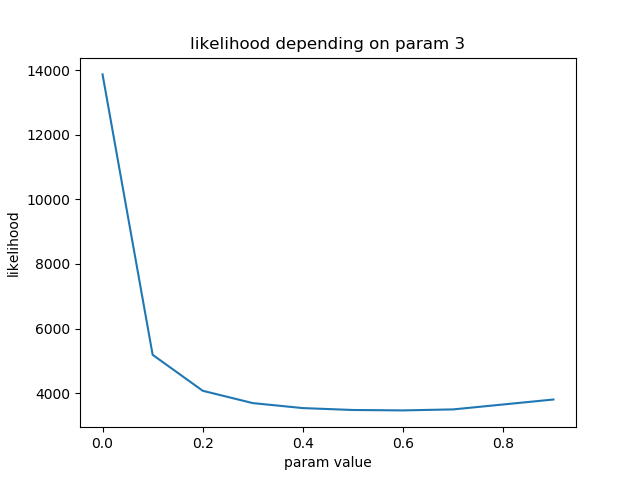
\includegraphics[scale=0.7]{../likelihoodPlot3DNMT3KO.png}
\label{rangedelta}
\caption{Negative log-likelihood depending on parameter $\delta$; the other three parameter values are fixed.}
\end{figure}

%mSat restrictions
We evaluate the likelihood function further by investigating the borders of the function. We thus compare the value of the likelihood after each parameter was set to zero and one to the present minimum. Further, during the \ac{MLE} computation, it was striking that sometimes some parameters were difficult to identify because the range where this parameter maximizes the likelihood was wide as visible in figure \ref{rangedelta}. Therefore, another approach was to fix an interval for the parameters, which may maximize the likelihood. The best results for the parameter restrictions for mSat are shown in row two and three in table \ref{DNMT1KO} and \ref{DNMT3KO}.\newline
For both methyltransferases, the likelihood is maximized by setting $\rho$ to one. $\tau$ and $\delta$ do not change significantly compared to the result without parameter restriction for DNMT3, while $\mu$ decreases by 0.217.\newline
For DNMT1 $\tau$ decreases and $\mu$ increases a bit such that all parameters besides $\delta$ are very high. Regularly, the interpretation of a high $\rho$ would be that the enzyme falls off at each \ac{bp}, but in this case, if $\tau$ is next to one too, the \ac{DNMT} will immediately bind again. In this model, the enzyme can be interpreted as very processive. We are not able to distinguish between a low disassociation probability and a very high dis- and reassociation probability as both combinations lead to the event that the methyltransferase is bound to one \ac{bp} and its successor. Thus, DNMT1 is interpreted as very processive and the result with $\rho=1$ and $\tau \approx 1$ is similar to the previous result.\newline
Another very likely scenario for DNMT3 is, if $\tau$ was set to one. Then $\rho$ is approximately one, but the methylation probabilities decrease compared to the approach without parameter restriction. The interpreting is different here, because the methylation activity is low. DNMT3 seems to work processive in this case but methylation events occur rather rarely.\newline
In the third scenario of DNMT1 and locus mSat, $\mu$ was restricted to the interval [0.8,1]. Compared to row one of table \ref{DNMT3KO}, both parameter estimations are very similar again; only the disassociation probability is even lower. Both results suggest a processive behaviour of DNMT1 with high methylation probabilities.\newline
In sum...

\subsection{Afp}
\label{Afp}

\subsection{IAP}
\label{IAP}

\subsection{WT}
\label{WT}
\begin{figure}[h]
\begin{center}
\begin{tabularx}{\textwidth}{l|c|c|c|c|c|c}
locus&	restrictions&	$\rho$&	$\tau$&	$\mu$&	$\delta$&	likelihood\\
\hline
mSat&	&	0.56&	0.872&	$\approx1$&	0.472&	3430\\
	&	&	0&	$\approx1$&	0.051&	0.572&	\\
\hline
Afp&	&	0.026&	0.96&	0.888&	$\approx1$&	1110\\
	&	&	0.419&	0.371&	0.797&	0.914&	\\
\hline
Afp&	$0 \leq \delta1 \leq 0.3$&	0.301&	0.895&	1&	0.18&	1077\\%**
	&	&	0.988&	0.858&	$\approx0$&	$\approx1$&	\\
\hline
Afp&	$0 \leq \delta1 \leq 0.5 \wedge 0.8 \leq \delta3 \leq 1$&	0.379&	0.915&	$\approx1$&	0.5&	1056\\
	&	&	0.268&	0.754&	$\approx0$&	0.956&	\\
\hline
IAP&	&	0.416&	0.927&	0.963&	0.749&	1838\\%*
	&	&	0.708&	0.912&	0&	0.61&	\\
\hline
IAP&	$0 \leq \delta1 \leq 0.5$&	0.17&	0.876&	0.957&	$\approx0$&	1832\\%**
	&	&	0.575&	0.879&	$\approx0$&	$\approx1$&	\\
\end{tabularx}
\end{center}
\label{WT33}
\caption{Parameter for minimal negative log-likelihoods of three loci for WT after 33 cell divisions, the first row for every locus shows the parameter for DNMT1($\rho1, \tau1, \mu1, \delta1$); the second row for DNMT3($\rho3, \tau3, \mu3, \delta3$).}
\end{figure}

\begin{figure}[h]
\begin{center}
\begin{tabularx}{\textwidth}{l|c|c|c|c|c|c}
locus&	restrictions&	$\rho$&	$\tau$&	$\mu$&	$\delta$&	likelihood\\
\hline
mSat&	&	1&	0.907&	1&	0.701&	3660\\%X
	&	&	1&	0.053&	0&	0&	\\
\hline
mSat&	$0 \leq \rho1 \leq 0.2 \wedge 0.4 \leq \rho3 \leq 1$&	0.2&	1&	0.89&	0.284&	3449\\%**
	&	$\wedge 0.5 \leq \delta3 \leq 1$&	1&	0.584&	0.286&	0.694&	\\
\hline
Afp&	&	$\approx0$&	0.916&	0.87&	$\approx0$&	3510\\
	&	&	0.971&	0.963&	0.399&	0.748&	\\
\end{tabularx}
\end{center}
\label{WT33}
\caption{Parameter for minimal negative log-likelihoods of three loci for WT after 100 cell divisions, the first row for every locus shows the parameter for DNMT1($\rho1, \tau1, \mu1, \delta1$); the second row for DNMT3($\rho3, \tau3, \mu3, \delta3$).}
\end{figure}

\section{Approximative Bayesian Computation}
\label{ABC}
\chapter{Conclusions}
\label{chapter:conclusions}

todo
\appendix
\chapter{Regulation}
\label{section:reg_appendix}


% bibliography
\cleardoublepage
\addcontentsline{toc}{chapter}{Bibliography}
\printbibliography
\vfill

\end{document}

